% =============================================================================
% The CGAL Developers' Manual
% Chapter: Reference Counting and Handle Types
% -----------------------------------------------------------------------------
% file   : handles.tex
% authors: Stefan Schirra <stschirr@mpi-sb.mpg.de>
% -----------------------------------------------------------------------------
% $Id$
% $Date$
% =============================================================================

\chapter{Reference Counting and Handle Types\label{chap:reference_counting}}

\ccChapterAuthor{Stefan Schirra ({\tt stschirr@mpi-sb.mpg.de})}

\section{Reference counting}
As of release 2.1, a reference counting%
\ccIndexMainItem{reference counting} scheme is used for
the kernel objects in the kernels \ccc{Cartesian}\ccIndexSubitem{kernel}{\ccFont Cartesian} and 
\ccc{Homogeneous}\ccIndexSubitem{kernel}{\ccFont Homogeneous}. 
All copies of an object share a common representation object storing
the data associated with a kernel object; see Figure~\ref{fig:refcounted}.

The motivation is to save space by avoiding storing the same data more 
than once and to save time in the copying procedure. 
Of course, whether we actually save time and space depends on the size 
of the data that we would have to copy without sharing representations.
The drawback is an indirection in accessing the data. Such an indirection is 
bad in terms of cache efficiency.\ccIndexMainItem{cache efficiency} 
Thus there are also non-reference-counting kernels available
\ccc{Simple_cartesian} and \ccc{Simple_homogeneous}.

\begin{figure}
\lcTex{
\begin{center}
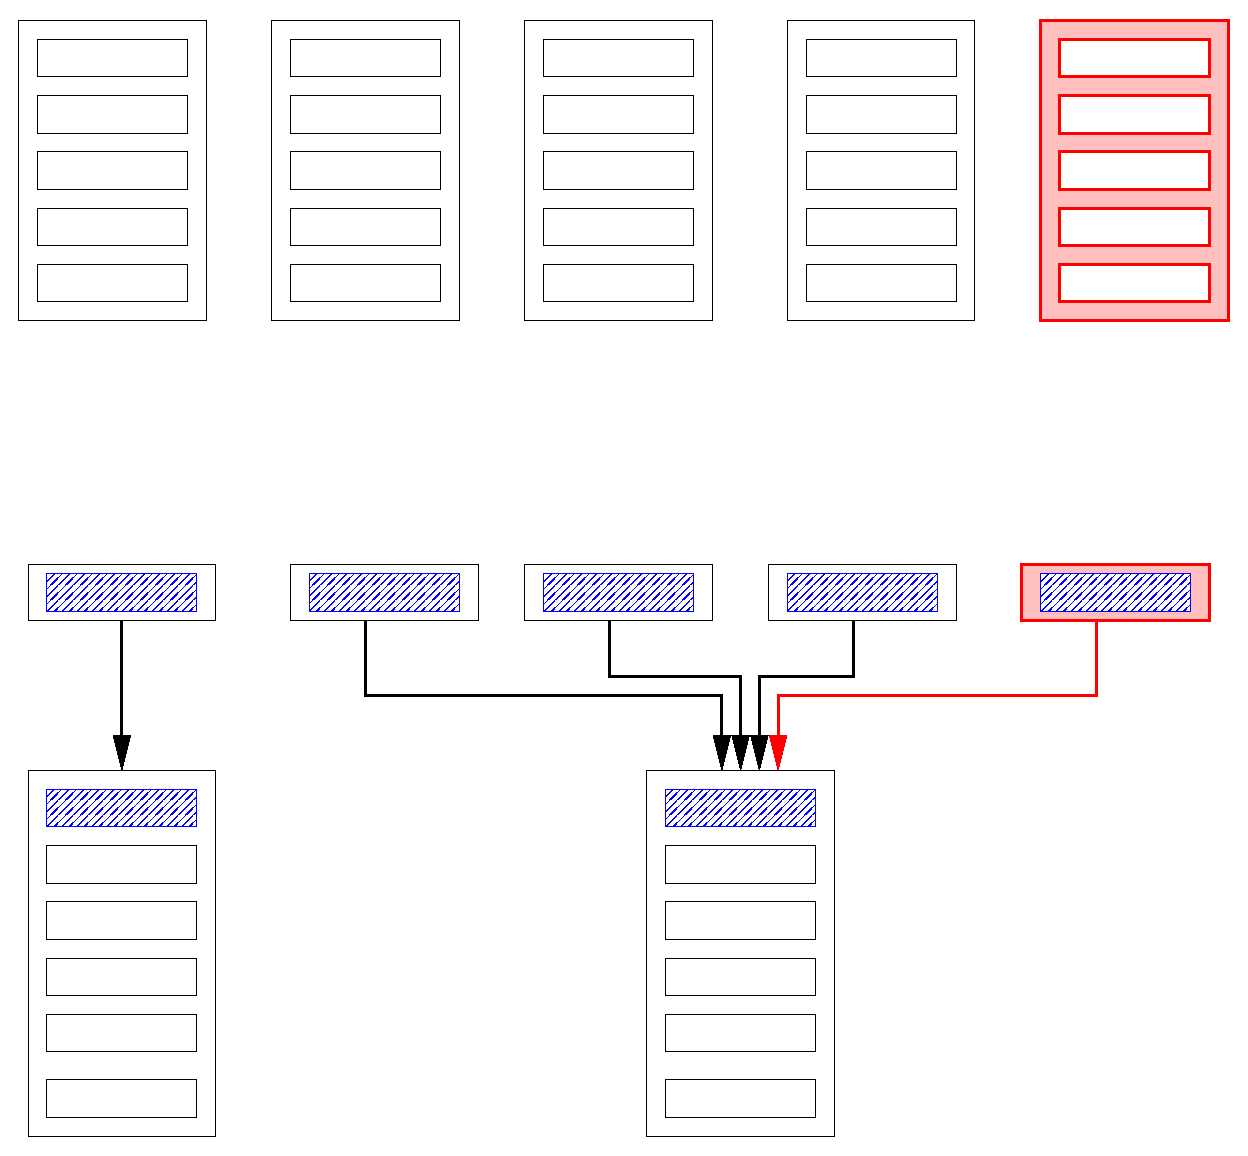
\includegraphics[width=0.6\textwidth]{Developers_manual/fig/reference_counting}
\end{center}
}
\caption{Objects using reference counting (bottom) share common representation;
copying creates a new handle (drawn at the right) pointing to the same 
representation as the object copied. Without reference counting (top) 
all data are copied to the new object (drawn at the right);\label{fig:refcounted}} 
\lcRawHtml{
<CENTER>
<IMG BORDER=0 src="fig/reference_counting.gif"
   ALT="Reference counted objects"><BR>
</CENTER>
}
\end{figure}


The reference counting in the kernel objects is not visible to a user
and does not affect the interface of the objects. 
The representation object is often called
the {\em body}%
\ccIndexSubitem{reference counting}{body}.
The object possibly sharing its representation with others
is called a {\em handle}\ccIndexSubitem{reference counting}{handle},
because its data consists of a pointer
to its representation object only. If the implementation of the member 
functions is located with the representation object and the functions in the 
handle just forward calls to the body, the scheme implements the {\em bridge}
design pattern,\ccIndexMainItem{bridge design pattern}
which is used to separate an interface from its implementation.
The intent of this design pattern is to allow for exchanging implementations
of member functions hidden to the user, especially at runtime. 

\section{Handle \& Rep}
The two classes \ccc{Handle}\ccIndexMainItem[C]{Handle} and 
\ccc{Rep}\ccIndexMainItem[C]{Rep} provide reference counting
functionality; see Figure \ref{fig:HandleRep}. By deriving from these classes, 
the reference counting functionality is inherited. 
The class \ccc{Rep} provides a counter; representation classes 
derive from this class. 
The class \ccc{Handle} takes care of all the reference-counting
related stuff. In particular, it provides appropriate implementations of
copy constructor, copy assignment, and destructor. These functions
take care of the counter in the common representation. 
Classes sharing reference-counted 
representation objects (of a class derived from \ccc{Rep}) do not have to
worry about the reference counting, with the exception of non-copy-constructors.
\ccIndexSubitem{constructor}{for classes sharing reference-counted objects}
There  a new representation object must be created and the pointer to the 
representation object must be set.

If \ccc{CGAL_USE_LEDA}%
\index{CGAL_USE_LEDA flag@{\tt CGAL\_USE\_LEDA} flag}
is defined and \ccc{CGAL_NO_LEDA_HANDLE}%
\index{CGAL_NO_LEDA_HANDLE flag@{\tt CGAL\_NO\_LEDA\_HANDLE} flag} is not
defined, the types \ccc{Handle} and \ccc{Rep} are set to the \leda\ types
\ccc{handle_base}%
\ccIndexMainItem[C]{handle_base} and \ccc{handle_rep}%
\ccIndexMainItem[C]{handle_rep}, respectively (yes, 
without a \ccc{leda_}-prefix). Use of the \leda\ class \ccc{handle_rep} implies
that \leda\ memory management\ccIndexSubitem{\leda}{memory management}
is used for the representation types.

\begin{verbatim}
typedef handle_base      Handle;
typedef handle_rep       Rep;
\end{verbatim}

Scavenging \leda, we provide the identical functionality in the \cgal\ classes
\ccc{Leda_like_handle}%
\ccIndexMainItem[C]{Leda_like_handle} and \ccc{Leda_like_rep}%
\ccIndexMainItem[C]{Leda_like_rep}. If \leda\ is not available or
\ccc{CGAL_NO_LEDA_HANDLE} is set, \ccc{Handle} and \ccc{Rep} correspond to
these types.

\begin{verbatim}
typedef Leda_like_handle Handle;
typedef Leda_like_rep    Rep;
\end{verbatim}

\begin{figure}[ht]
\lcTex{
\begin{center}
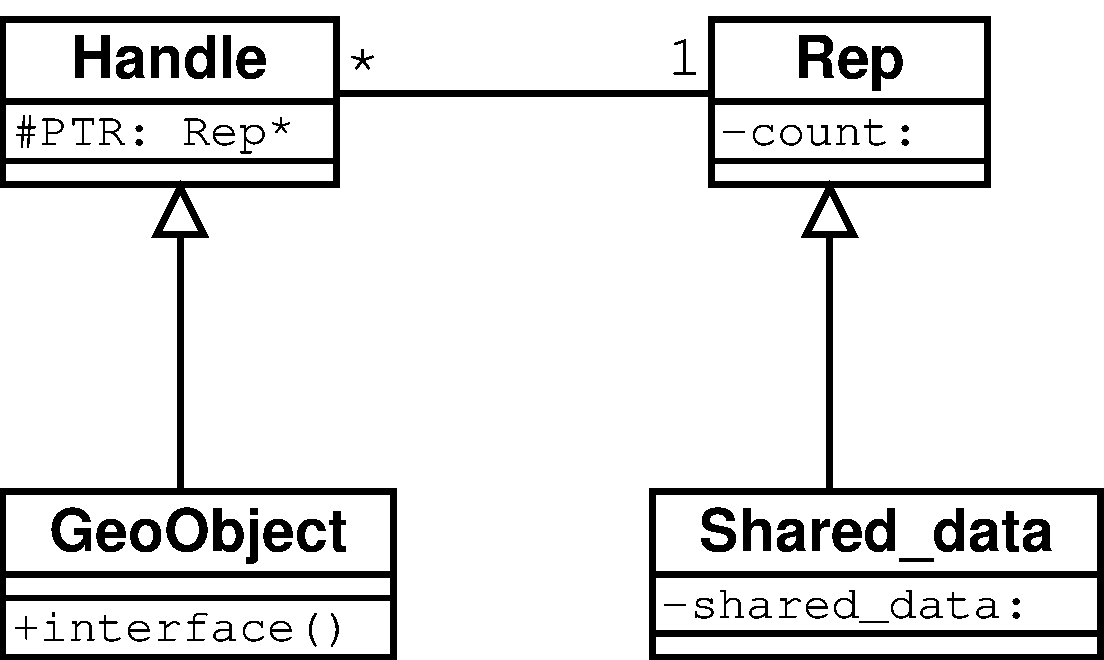
\includegraphics[width=7cm]{Developers_manual/fig/handle_rep}
\end{center}
}
\caption{UML class diagram for Handle \& Rep scheme.\label{fig:HandleRep}}
\lcRawHtml{
<CENTER>
<IMG BORDER=0 SRC="fig/handle_rep.gif" 
  ALT="Handle & Rep UML class diagram"><BR>
</CENTER>
}
\end{figure}

\section{Using Handle \& Rep}
In order to make use of the reference counting provided by the
classes \ccc{Handle} and \ccc{Rep}, your interface class (the class providing
the interface of the geometric object) must be derived from \ccc{Handle} and
your representation class (the class containing the data to be shared) must be 
derived from \ccc{Rep}:

\begin{verbatim}
class My_rep : public Rep { /*...*/ };
class My_geo_object : public Handle 
{
  public:
    My_geo_object(const My_geo_object& m);

    My_geo_object(Arg1, Arg2);
};
\end{verbatim}

The class \ccc{My_geo_object} is responsible for allocating and constructing
the \ccc{My_rep} object ``on the heap''. 
Typically, a constructor call is forwarded to a
corresponding constructor of \ccc{My_rep}. The address of the new \ccc{My_rep}  is assigned to \ccc{PTR} inherited from \ccc{Handle}, e.g.:

\begin{verbatim}
My_geo_object::My_geo_object(Arg1 a1, Arg2 a2)
{ PTR = new My_rep(a1, a2); }
\end{verbatim}

The default constructor of \ccc{Handle} is called automatically
by the compiler and the reference counting is initialized. 
You always have to define a copy constructor for \ccc{My_geo_object} 
\ccIndexSubitem{copy constructor}{for Handle-derived class}
and to call the copy constructor of \ccc{Handle} there:

\begin{verbatim}
My_geo_object::My_geo_object(const My_geo_object& m)
 : Handle( m) 
{}
\end{verbatim}

That's it!
There is no need to define a copy assignment operator nor is there a 
need to define a destructor for the derived class \ccc{My_geo_object}!  
Handle \& Rep does the rest for you!
You get this functionality by

\ccInclude{CGAL/Handle.h}

It is common practice to add a (protected) member function \ccc{ptr()}
to the class \ccc{My_geo_object},
which casts the \ccc{PTR} pointer from \ccc{Rep*} to the actual type
\ccc{My_rep*}. 

Note that this scheme is meant for non-modifiable types. You are not allowed
to modify data in the representation object, because the data are possibly
shared with other \ccc{My_geo_object} objects.

\section{Templated handles}
Factoring out the common functionality in base classes enables re-use of 
the code, but there is also a major drawback. The \ccc{Handle} class does not
know the type of the representation object. It maintains a \ccc{Rep*} pointer.
Therefore, this pointer must be cast to a pointer to the actual type
in the classes derived from \ccc{Handle}. Moreover, since the \ccc{Handle}
calls the destructor for the representation through a \ccc{Rep*}, the
destructor of \ccc{Rep} must be virtual. Finally, debugging is difficult,
again, because the \ccc{Handle} class does not know the type of the 
representation object.
Making the actual type of the representation object a template parameter
of the handle solves these problems. This is implemented in class template
\ccc{Handle_for}.%
\ccIndexMainItem[C]{Handle_for} 
This class assumes that the reference-counted class provides the
following member functions
to manage its internal reference counting: 
\def\ccIndexClassName{Ref_counted}
\begin{itemize}
\item\ccc{add_reference}\ccIndexMemberFunction{remove_reference}
\item\ccc{remove_reference}\ccIndexMemberFunction{remove_reference}
\item\ccc{bool is_referenced}\ccIndexMemberFunction{is_referenced}
\item\ccc{bool is_shared}\ccIndexMemberFunction{is_shared}
\end{itemize}
See the UML class diagram in Figure \ref{fig:HandleFor}.
The reference counting functionality and the required
interface can be inherited from class \ccc{Ref_counted}.
\ccIndexMainItem[C]{Ref_counted} 

\begin{figure}[ht]
\lcTex{
\begin{center}
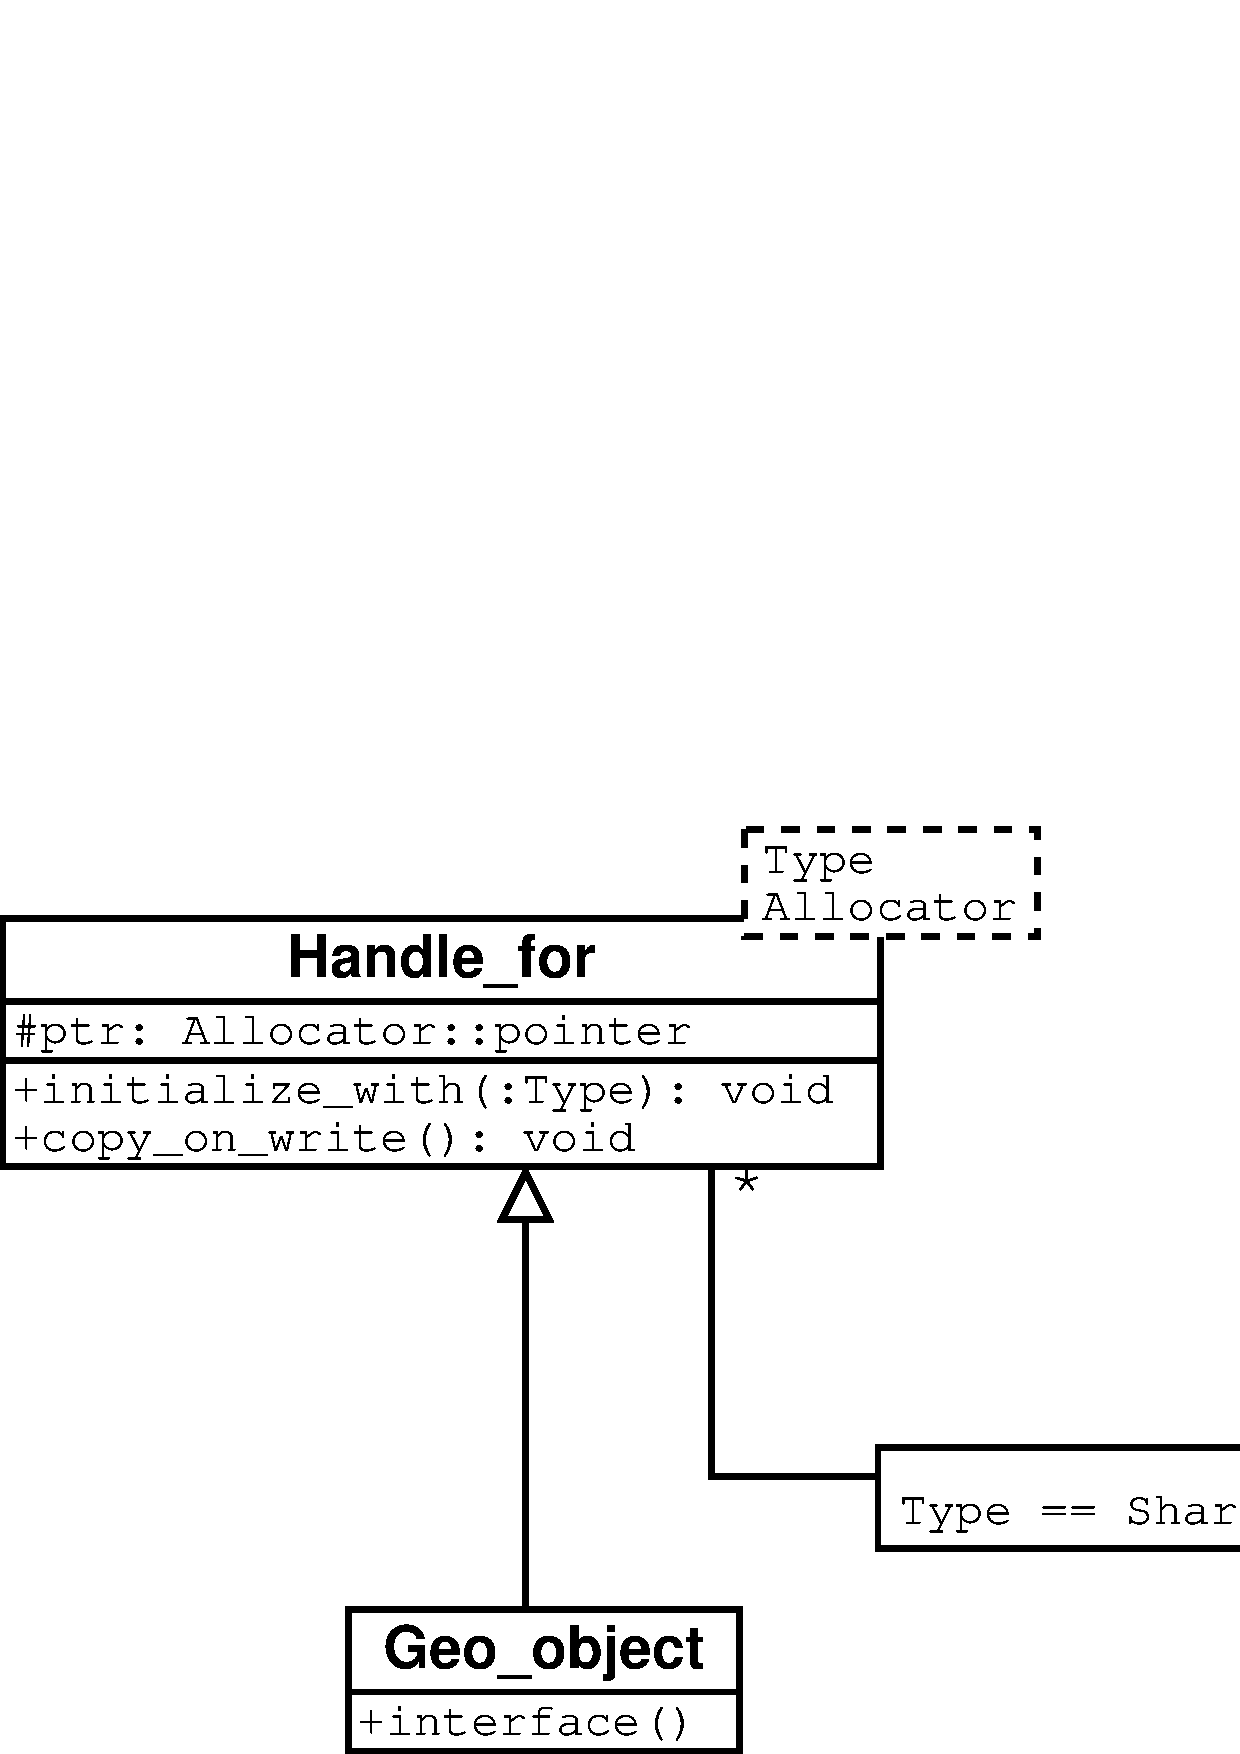
\includegraphics[width=13.5cm]{Developers_manual/fig/handle_allocate}
\end{center}
}
\caption{UML diagram for templated handles.\label{fig:HandleFor}}
\lcRawHtml{
<CENTER>
<IMG BORDER=0 SRC="fig/handle_allocate.gif"
   ALT="Templated handles UML diagram"><BR>
</CENTER>
}
\end{figure}

Kernel objects have used such a handle/rep scheme since release 2.2. 

\section{Using templated handles}
In order to make use of the reference counting provided by the
classes \ccc{Handle_for} and \ccc{Ref_counted}, your representation class, 
let's say \ccc{My_rep} (the class containing the data to be shared), 
must provide the interface described above (\eg, by deriving 
from \ccc{Ref_counted}), and your interface class (the class providing
the interface of the geometric object) must be derived from 
\ccc{Handle_for<My_rep>}. It is assumed that the default constructor of
\ccc{My_rep} sets the counter to 1 (the default constructor of 
\ccc{Ref_counted} does this, of course): 

\begin{verbatim}
class My_rep : public Ref_counted { /*...*/ };

class My_geo_object : public Handle_for<My_rep> 
{
  public:
    My_geo_object(const My_geo_object& m);

    My_geo_object(Arg1, Arg2);
};
\end{verbatim}

You should also define a copy constructor for \ccc{My_rep} as this may be used 
in in-place creation in the allocator scheme.
The constructors of class \ccc{My_geo_object} are responsible for constructing
the \ccc{My_rep} object. 
%The space for the object is allocated
%by \ccc{Handle_for}, so construction is done by an in-place new
%operation at the location pointed to by \ccc{ptr}. 
Typically, a corresponding constructor call of \ccc{My_rep} is forwarded 
to \ccc{Handle_for}.

\begin{verbatim}
My_geo_object::My_geo_object(Arg1 a1, Arg2 a2)
 : Handle_for<My_rep>( My_rep(a1, a2)) {}
\end{verbatim}

Sometimes, you have to do some calculation first before you can
create a representation object in a constructor of \ccc{My_rep}.
\def\ccIndexClassName{Handle_for}
Then you can use the \ccc{initialize_with()}%
\ccIndexMemberFunction{initialize_with} member function
of \ccc{Handle_for}. 

In both cases, \ccc{Handle_for} takes care of allocating space for
the new object. 

If you define a copy constructor for \ccc{My_geo_object} 
you have to call the copy constructor of \ccc{Handle_for} there:

\begin{verbatim}
My_geo_object::My_geo_object(const My_geo_object& m)
 : Handle_for<My_rep>( m) 
{}
\end{verbatim}

That's it! Again, there is no need to define a copy assignment operator 
nor is there a need to define a destructor for the derived class 
\ccc{My_geo_object}!  \ccc{Handle_for} does the rest for you!

\ccc{Handle_for} provides you with an option to modify the data. There is
a \ccc{copy_on_write()}\ccIndexMemberFunction{copy_on_write} 
that should be called right before every modification of the data. 
It ensures that only your data are overwritten: 

\begin{verbatim}
void 
My_geo_object::set_x(double d)
{
  copy_on_write();
  ptr->x = d;
}
\end{verbatim}
You get this functionality by

\ccInclude{CGAL/Handle_for.h}

\section{Allocation}
Class \ccc{Handle_for} has two template parameters. Besides the
type of the stored object, there is also a parameter specifying an
allocator.\ccIndexMainItem{allocator}
Any concrete argument must be a model for the \ccc{Allocator} concept
defined in the \CC\ standard. There is a default value for the second
parameter defined as \ccc{CGAL_ALLOCATOR(T)}. But you can also choose your
own, for example

\begin{verbatim}
class My_geo_object : public Handle_for<My_rep, leda_allocator<My_rep> > 
{ /* ... */ };
\end{verbatim}

The default allocator is defined in

\ccInclude{CGAL/memory.h}

See Chapter \ref{chap:memory_management} for more information.

